\chapter{Objective 2}

\section{Introduction}

{\color{codegreen}Jewel Loggings} (located in the Castle Approach area), greeted our heroes. He mentioned that helping elves gives hints
and also to pick up various objects lying around.

- Why do we need to bother ourselves picking random trash?

- It may not be trash, we may need it to help Santa.

- Yeah, I just finished reading all of Marie Kondo's books and rearranged my condo.

- Grinch, I was begging you for months to clean up your desk drawers and you wouldn't do it. Don't play me the Kondo card now.
You can manage for a few hours.

- Fair enough Cindy Lou, fair enough. Anyway, we need to find some solution regarding those buckets.
\newline
{\color{codegreen}Shinny Uppatree} (located in the Castle Approach area) was there hanging by a terminal, waiting for someone to save the day.
The elf asked us to take a look at \textit{Kringle Kiosk}. He has reason to believe that there is some sort of command injection bug there.

Cindy Lou, colloquially known as "walking zero-day machine" decided to take a look.

\subsection{Kringle Kiosk}
This is a challenge that requires us to escape to \textit{/bin/bash}.
If we select option 4, we are greeted by \href{https://en.wikipedia.org/wiki/Cowsay}{Cowsay}
\begin{figure}[h!]
  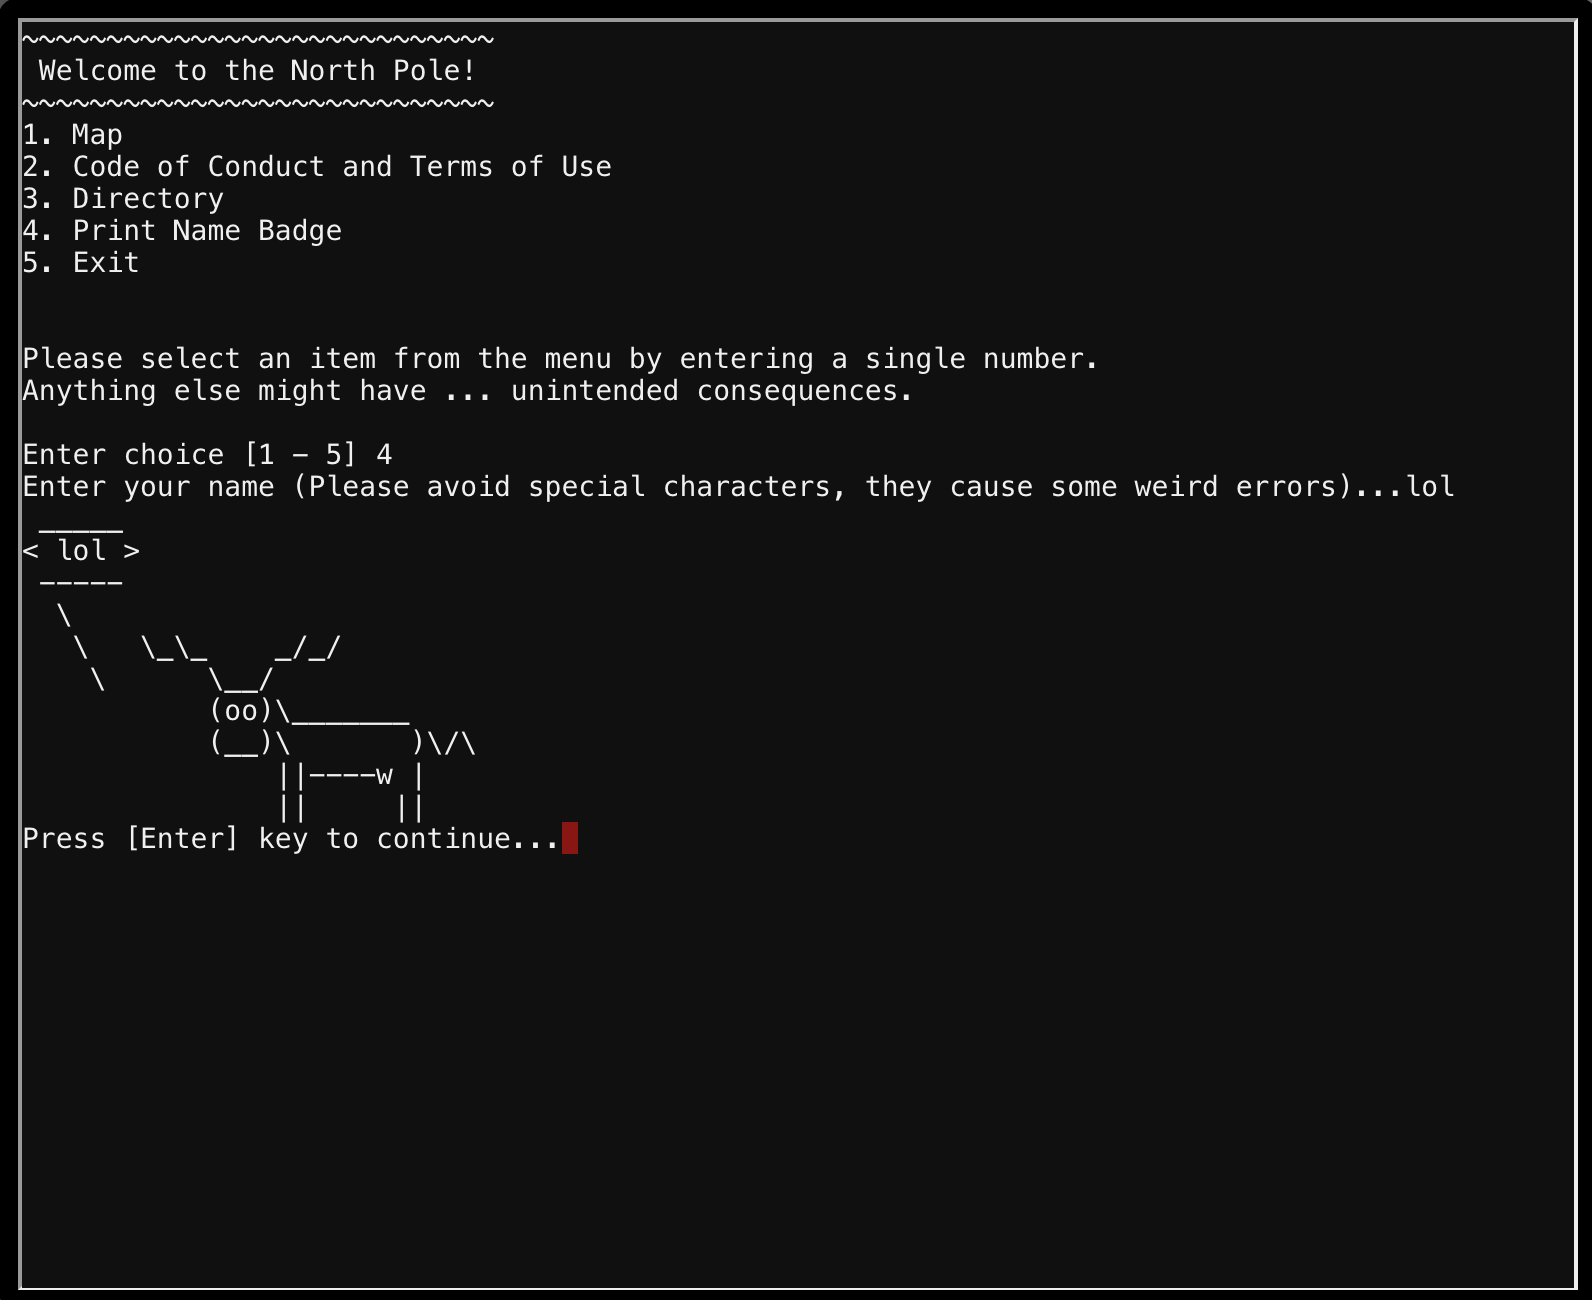
\includegraphics[scale=0.5]{kk-cow}
  \caption{Printscreen of Kringle Kiosk challenge}
\end{figure}

\newpage
Cindy Lou assumed that the code running in the background looked like:

\begin{minted}{bash}
$ cowsay $USER_INPUT
\end{minted}

Escaping can happen in many ways but Cindy decided to try the following:
\begin{minted}{bash}
  $ ; /bin/bash
\end{minted}

which worked.
\newpage
\begin{figure}[h!]
  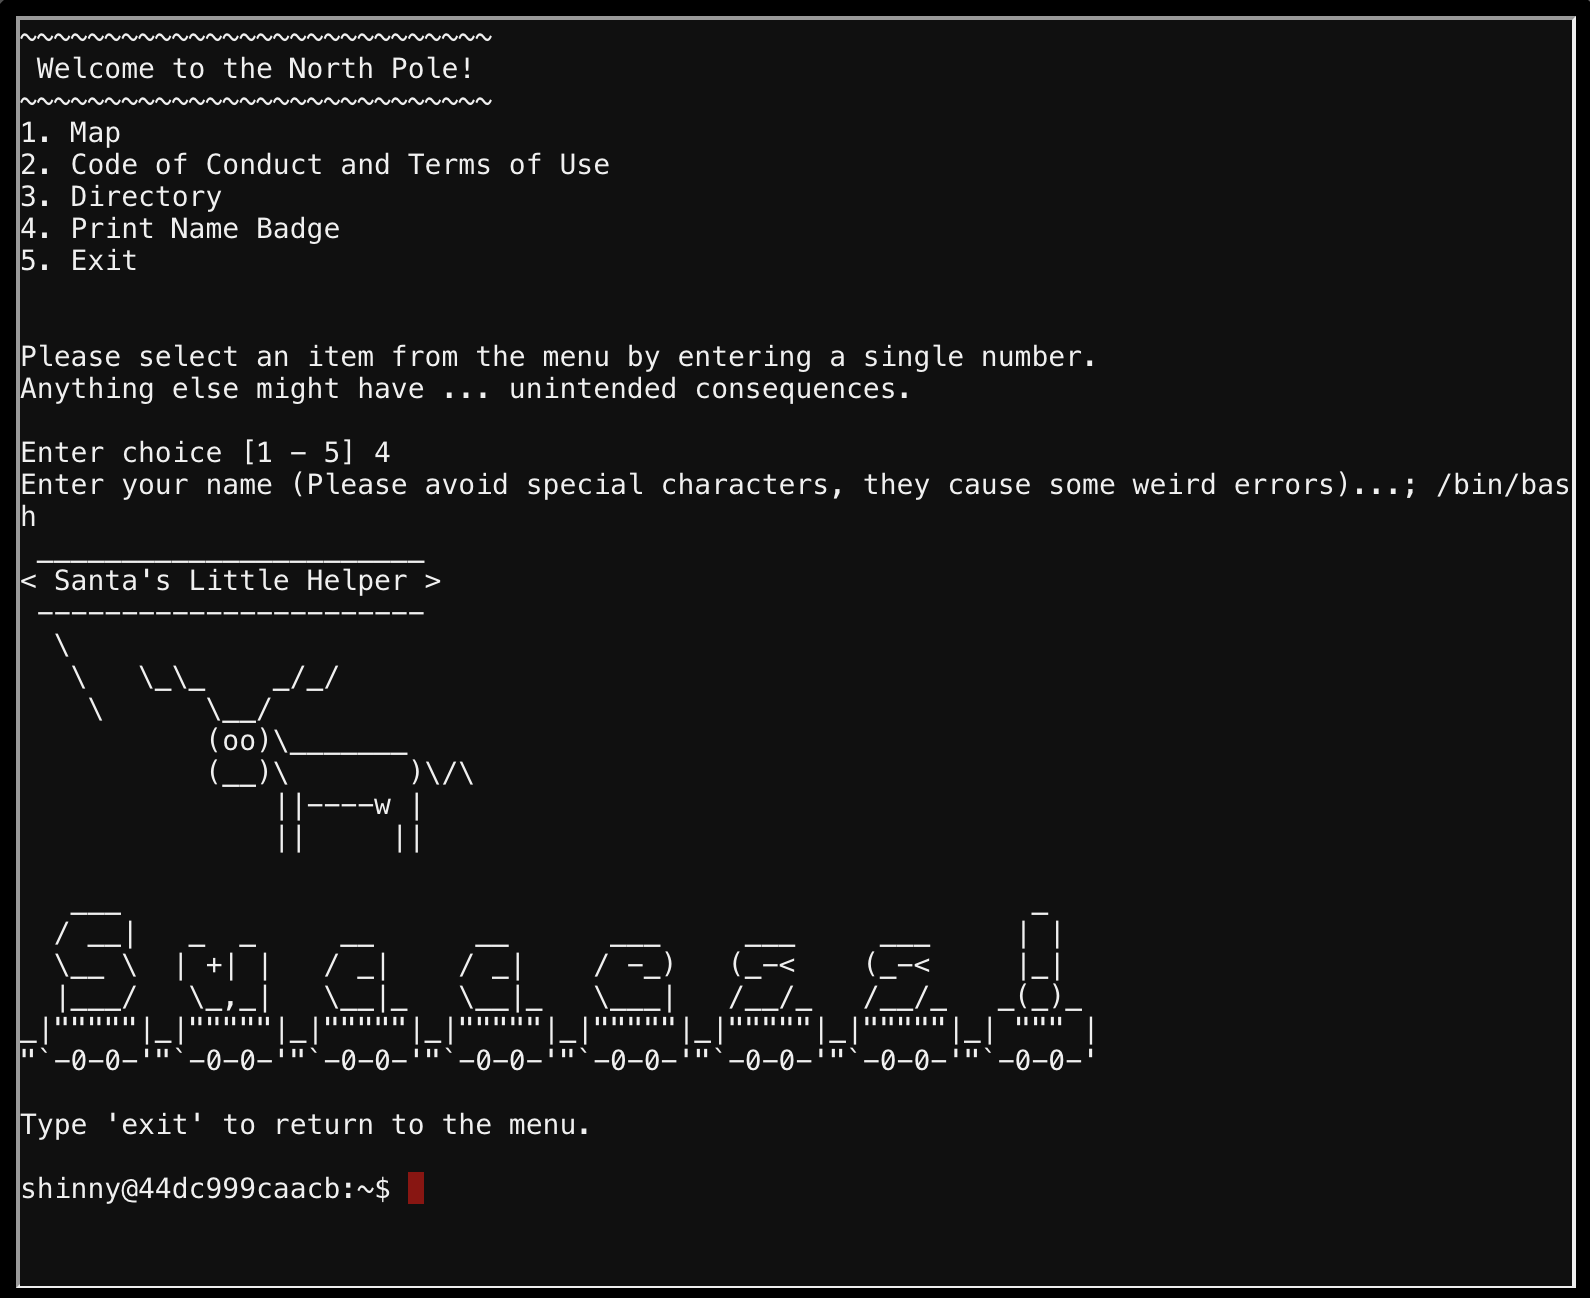
\includegraphics[scale=0.5]{kk-cow-escape}
  \caption{Printscreen of Kringle Kiosk escape.}
\end{figure}

{\color{codegreen}Shinny Uppatree} excited that the flaw was found, asked if we could take a look at finding a bucket and identifying the \textit{package}.
He mentioned briefly that he believes that the package is reversible. When opening the challenge, we are also hinted about \textit{Wrapper3000} which is the latest and greatest
tool in obfuscation.

Cindy went ahead and typed quickly. She was fairly familiar with S3 buckets, having identified multiple issues in the past. She enriched her wordlist based on the discussion with the elves.
\begin{minted}{bash}
elf@d26fd59a0911:~$ cd bucket_finder/
elf@d26fd59a0911:~/bucket_finder$ ls
README  bucket_finder.rb  wordlist
elf@d26fd59a0911:~/bucket_finder$ echo Wrapper3000 >> wordlist
elf@d26fd59a0911:~/bucket_finder$ echo wrapper3000 >> wordlist
elf@d26fd59a0911:~/bucket_finder$ ruby bucket_finder.rb wordlist
http://s3.amazonaws.com/kringlecastle
Bucket found but access denied: kringlecastle
http://s3.amazonaws.com/wrapper
Bucket found but access denied: wrapper
http://s3.amazonaws.com/santa
Bucket santa redirects to: santa.s3.amazonaws.com
http://santa.s3.amazonaws.com/
      Bucket found but access denied: santa
http://s3.amazonaws.com/Wrapper3000
Bucket does not exist: Wrapper3000
http://s3.amazonaws.com/wrapper3000
Bucket Found: wrapper3000 ( http://s3.amazonaws.com/wrapper3000 )
      <Public> http://s3.amazonaws.com/wrapper3000/package
elf@d26fd59a0911:~/bucket_finder$
\end{minted}

Sure enough, the \textit{wrapper3000} was the right bucket.
If we use the \textit{-d} option of the given tool it will download the files for us.
Cindy Lou's approach was to identify the contents and act accordingly.
\begin{minted}{bash}
738f5b259f0:~/$ file package
package: ASCII text, with very long lines
elf@obj2:~/$ cat package
UEsDBAoAAAAAAIAwhFEbRT8anw <snip> AAAAA # This looks like base64
elf@obj2:~/$ cat package | base64 -d # Let's try to decode it as B64 which works.
PK
<snip> package.txt.Z.xz.xxd.tar.bz2UT  <snip> _ux
elf@obj2:~/$ cat package | base64 -d > package.txt.Z.xz.xxd.tar.bz2UT
elf@obj2:~/$ ls
package  package.txt.Z.xz.xxd.tar.bz2UT
elf@obj2:~/$ file package.txt.Z.xz.xxd.tar.bz2UT # Identify package
package.txt.Z.xz.xxd.tar.bz2UT: Zip archive data, at least v1.0 to extract
elf@obj2:~/$ unzip package.txt.Z.xz.xxd.tar.bz2UT # Unzip
Archive:  package.txt.Z.xz.xxd.tar.bz2UT
  extracting: package.txt.Z.xz.xxd.tar.bz2
elf@obj2:~/$ file package.txt.Z.xz.xxd.tar.bz2 # Identify contents
package.txt.Z.xz.xxd.tar.bz2: bzip2 compressed data, block size = 900k
elf@obj2:~/$ bunzip2 package.txt.Z.xz.xxd.tar.bz2
elf@obj2:~/$ ls
package  package.txt.Z.xz.xxd.tar  package.txt.Z.xz.xxd.tar.bz2UT
elf@obj2:~/$ file package.txt.Z.xz.xxd.tar # Identify contents
package.txt.Z.xz.xxd.tar: POSIX tar archive
elf@obj2:~/$ tar xvf package.txt.Z.xz.xxd.tar
package.txt.Z.xz.xxd
elf@obj2:~/$ file package.txt.Z.xz.xxd # ASCII
package.txt.Z.xz.xxd: ASCII text
elf@obj2:~/$ cat package.txt.Z.xz.xxd # Inspect contents
<snip>
elf@obj2:~/$ xxd -r package.txt.Z.xz.xxd > package.txt.Z.xz
elf@obj2:~/$ xz -d package.txt.Z.xz # All extensions match, hit it
elf@obj2:~/$ file package.txt.Z
package.txt.Z: compress'd data 16 bits
elf@obj2:~/$ compress -d package.txt.Z
elf@obj2:~/$ cat package.txt
North Pole: The Frostiest Place on Earth # Answer
elf@obj2:~/$
\end{minted}

\subsection {On a more serious note}
\textit{Narrator's voice}. Although in my opinion AWS has great advantages, many companies "fail" to properly secure their assets (whether data or simply workloads).
AWS offers a wide variety of tools and IAM permissions that can be as fine-grained as you like. In my opinion, the more work and thought one puts in designing his cloud environment, the more pleasant it will be eventually.
From my experience, companies that have spent time designing AWS and generally building some sort of governance have serious benefits that extend security.
Infrastructure and Operations benefit, finance department is happy, developers get their little sandboxes of sorts to build stuff etc.

\subsection{Good 'ole tmux}
{\color{codegreen}Pepper Minstix} (located in the Castle Entrance), greeted our heroes. He needs to find his bird.
He must have detached his tmux \footnote{Tmux is a great tool and it's definitely worth the time to learn it and put in your daily routine.} session.
\begin{minted}{bash}
elf@8195fbf38e5d:~$ tmux list-sessions
0: 1 windows (created Sat Dec 26 20:04:55 2020) [80x24]
elf@8195fbf38e5d:~$ tmux attach-session -t 0
\end{minted}

He must have Ctrl+B-D.

\begin{figure}[h!]
  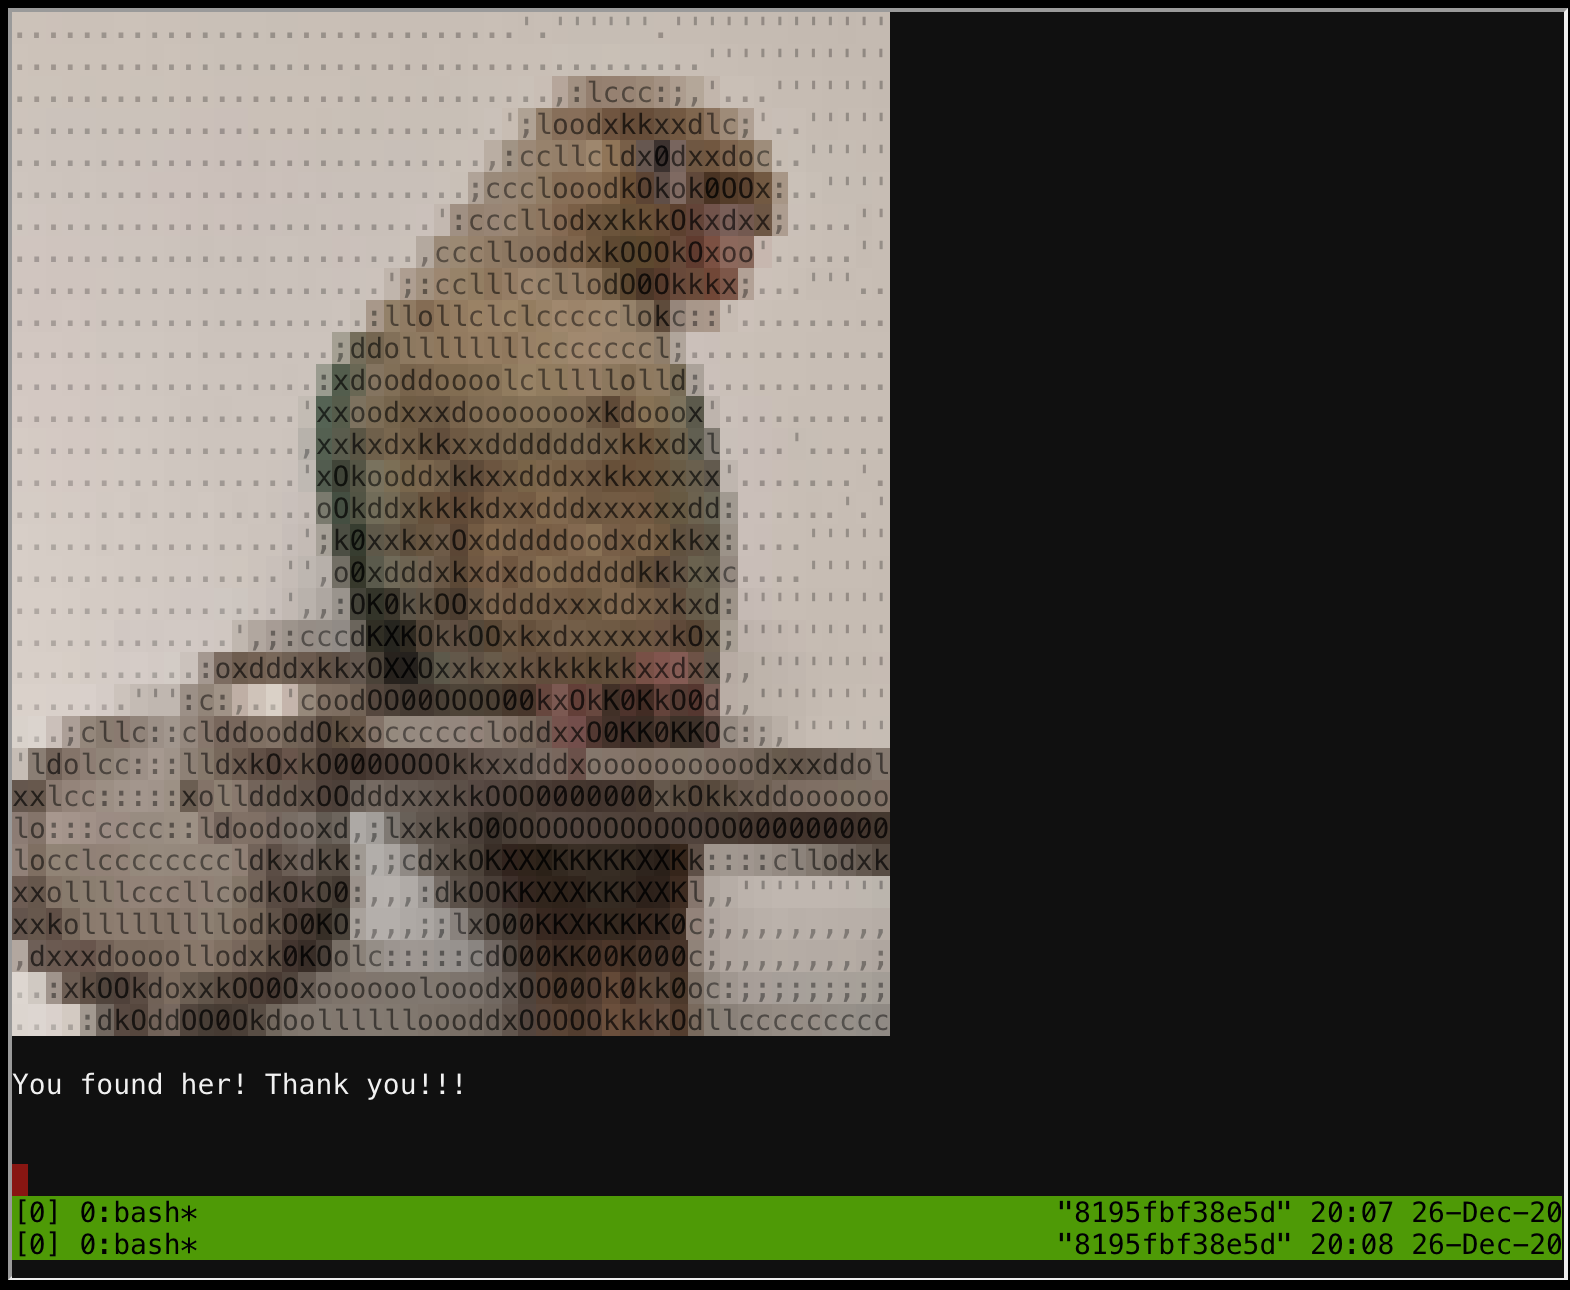
\includegraphics[scale=0.5]{tmux-solved}
  \caption{Printscreen of Tmux solution.}
\end{figure}

Based on Pepper's hints, we need to talk to {\color{codegreen}Sparkle Redberry} to get the key for the Santavator and also pick up objects.

Walking towards the castle, we find a \textit{Broken CandyCane}.
